\subsection{Biological Locomotion}
Locomotion is the combination of movement resulting in a progression from one location to another. Animal locomotion has evolved through natural selection to enable feeding, reproductive, anti-predator and habitat building behaviours. \cite{encyclopedia_locomotion_nodate}

Locomotion must first be separated into two main categories: active and passive Locomotion. Passive locomotion is  dependent on the environment. Typical animals showing this behaviours include jelly fish, spiders, insects, crustaceans and parasites. Wind, currents, tide and other natural energy are the main source of energy for passive locomotion. \cite{encyclopedia_locomotion_nodate}

Active locomotion enables animals to purposely progress from one location to another. Active locomotion can be separated into the five mediums found on earth: marine, fossorial, terrestrial, aboreal and aerial. \cite{encyclopedia_locomotion_nodate}

As the robot must use biomimetic locomotion, the following is a rapid review of limbs used by terrestrial animals. Figure \ref{fig:human} illustrate a homologous limb morphology comparison and Figure \ref{fig:insect} depicts the main differences in limbs used by insect and crustacean.

\begin{figure}[H]
    \centering
    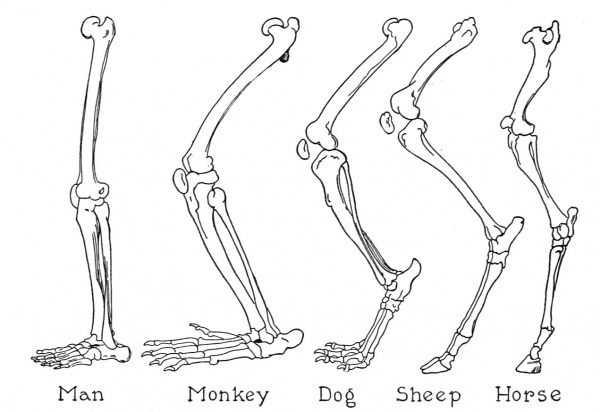
\includegraphics[width=0.35\textwidth]{Sections/LiteratureReview/img/Animals/humanLimbs.jpg}
    \caption{Comparative Homologous Structure \cite{tes_teach_comparative_nodate}}
    \label{fig:human}
\end{figure}

\begin{figure}[H]
    \centering
    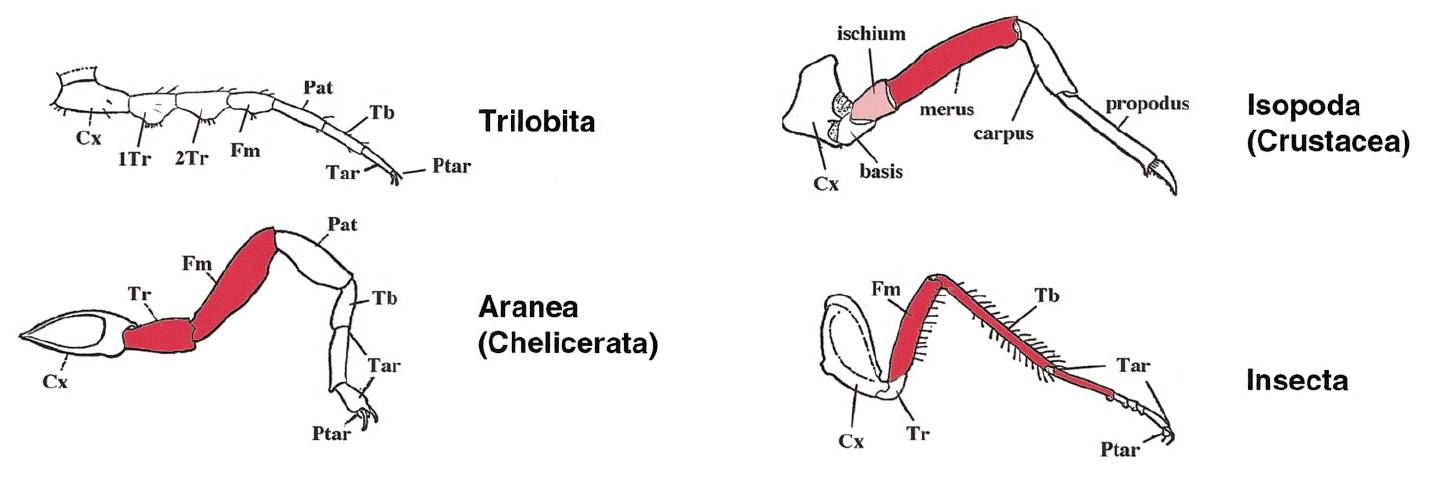
\includegraphics[width=0.6\textwidth]{Sections/LiteratureReview/img/Animals/InsectLimbs.png}
    \caption{Insect and Crustacean Limb Comparison \cite{abzhanov_fig._nodate}}
    \label{fig:insect}
\end{figure}



